%!TEX root = ../master.tex
\chapter{Design}\label{ch:design}
bla bla bla intro to chapter here hhhhhhhh jeg skriver lige noget her.

\section{An interactive board for Terra Mystica}
This project aims to create an interactive board for Terra Mystica, that uses Computer Vision to detect hand contact on the board via a camera below its surface. With the hand contact, the user should be able to change the colour of the hexagon-shaped tiles in the game. The idea is that the board itself is a projection from below, and the board should change according to inputs on the interaction with the board's surface.

The interactive board will eliminate the need for terrain game pieces, since it will manage terraforming digitally for the player. It may also assist the players in remembering the Power mechanic, as well as streamline other elements of the game.

A possible expansion of the project would be detection of game pieces, which can be used to measure amount of 'power' after game piece placement.

\section{Lo-fi test}
\begin{figure}
\centering 
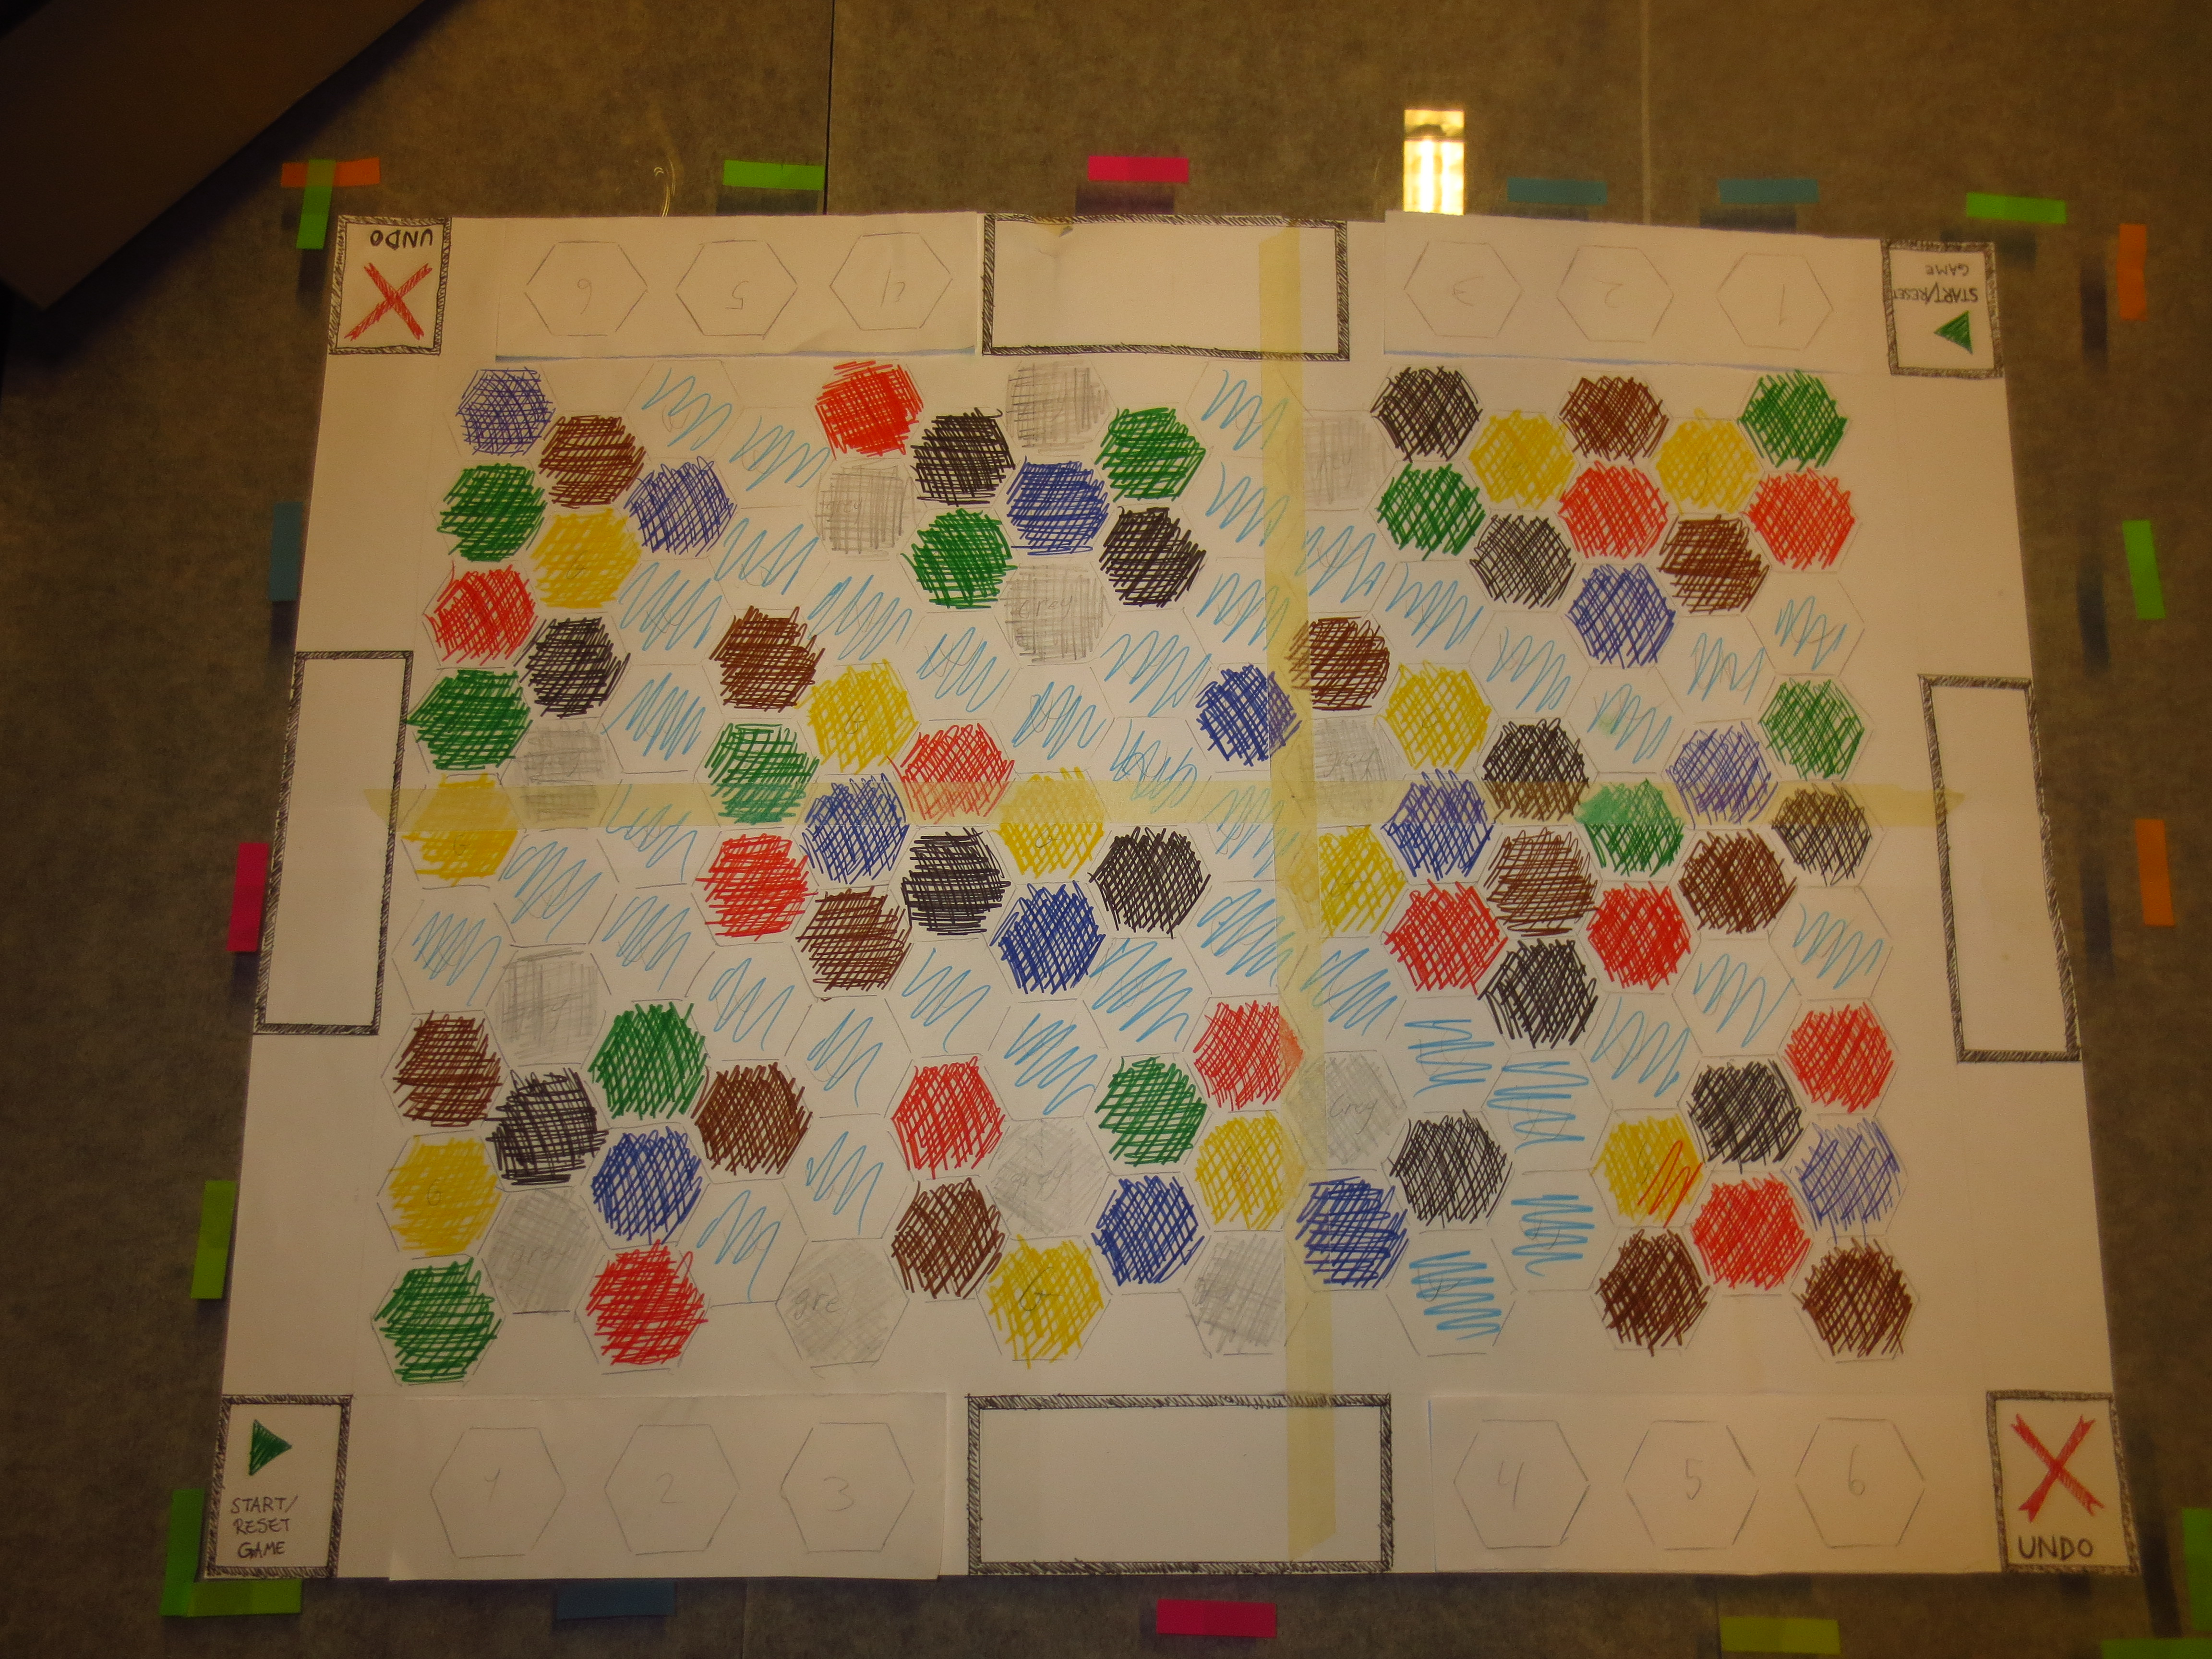
\includegraphics[width=0.9\textwidth]{IMG_0001}
\caption{The Lo-Fi board}
\end{figure} 

After defining the initial design a lo-fi test was conducted to test whether the areas of interest were large enough, the defined gestures were easy to perform and if the increased size had any effect on the gameplay. We also wanted a first outside opinion of the game without the terraforming pieces. 

For the lo-fi we had three participants: Nadia, Catja and Sebastian. \todo{Probably need their entire names here} 
They were all familiar with the game Terra Mystica so they did not need to learn the game first. They only played two rounds since one of the key points of the test was to learn if the gestures and the areas were good. 

They all had a little bit of trouble remembering to do the terraforming gesture in the beginning, but they were all pretty sure that with a little more playing it would come naturally/it would be fine. They also mentioned that it might be easier to remember to do the start of turn gesture if the non touch areas of the board lit up in their respective colours. 

They generally liked the bigger board since this made the hexes and other touch areas bigger, but they did also mention that for short people it might be a problem to reach the other end of the board. 

The mix of tangible and “digital” elements was confusing for the participants. They felt that it would make more sense to have the buildings digital but on the other hand they also felt that that would remove the tangibility that they like about the game. They mentioned that it might help to indicate where or when you want to build/upgrade since only doing a gesture whenever you need to terraform seems a bit odd. 

The personal player input area could be utilised better. Maybe it could indicate income or victory points or just indicate whenever it is your turn. 

The conclusions of the lo-fi test are that they gestures are easy to do and the areas of interest are large enough. The increased size of the board did make it harder for smaller players. The next step is then to discern if the programme will be able to recognise the gestures. 

\subsection{Procedure}
First participants were chosen from those who already knew the game.
Then they were introduced to the Lo-Fi board, by the primary interviewer who also acted as the "programme", about how the gestures worked and where they worked. They then played two rounds of the game, with some functions removed since they had no effect when only playing two rounds. During the game they commented out loud, which was noted down by the secondary interviewer who also noted down their reactions and behaviour. 
After the game they were asked some questions in a loosely structured group interview. 
The whole test was filmed. 